\section{Konzeptentwurf}
Bevor die Anwendung in die Cloud migriert werden kann, muss konzeptioniert werden, wie die Anwendungsarchitektur in Zukunft aussehen soll und wie diese final funktionieren wird. Dazu wurde vorangehend in der Anforderungsanalyse herausgearbeitet, welche Migrationsstrategie verfolgt werden soll und welche Voraussetzungen dafür geschaffen werden müssen.

Da die ursprüngliche Anwendung einige Funktionalitäten auf eine Weise umsetzt, die nicht in der Cloud funktionieren würde (z.B. das Lesen und Schreiben in Box), müssen diese überarbeitet oder neu geschrieben werden. Ein simples Rehosting ist durch die anfallenden Anpassungen entsprechend nicht möglich.

\begin{figure}[H]
    \centering
    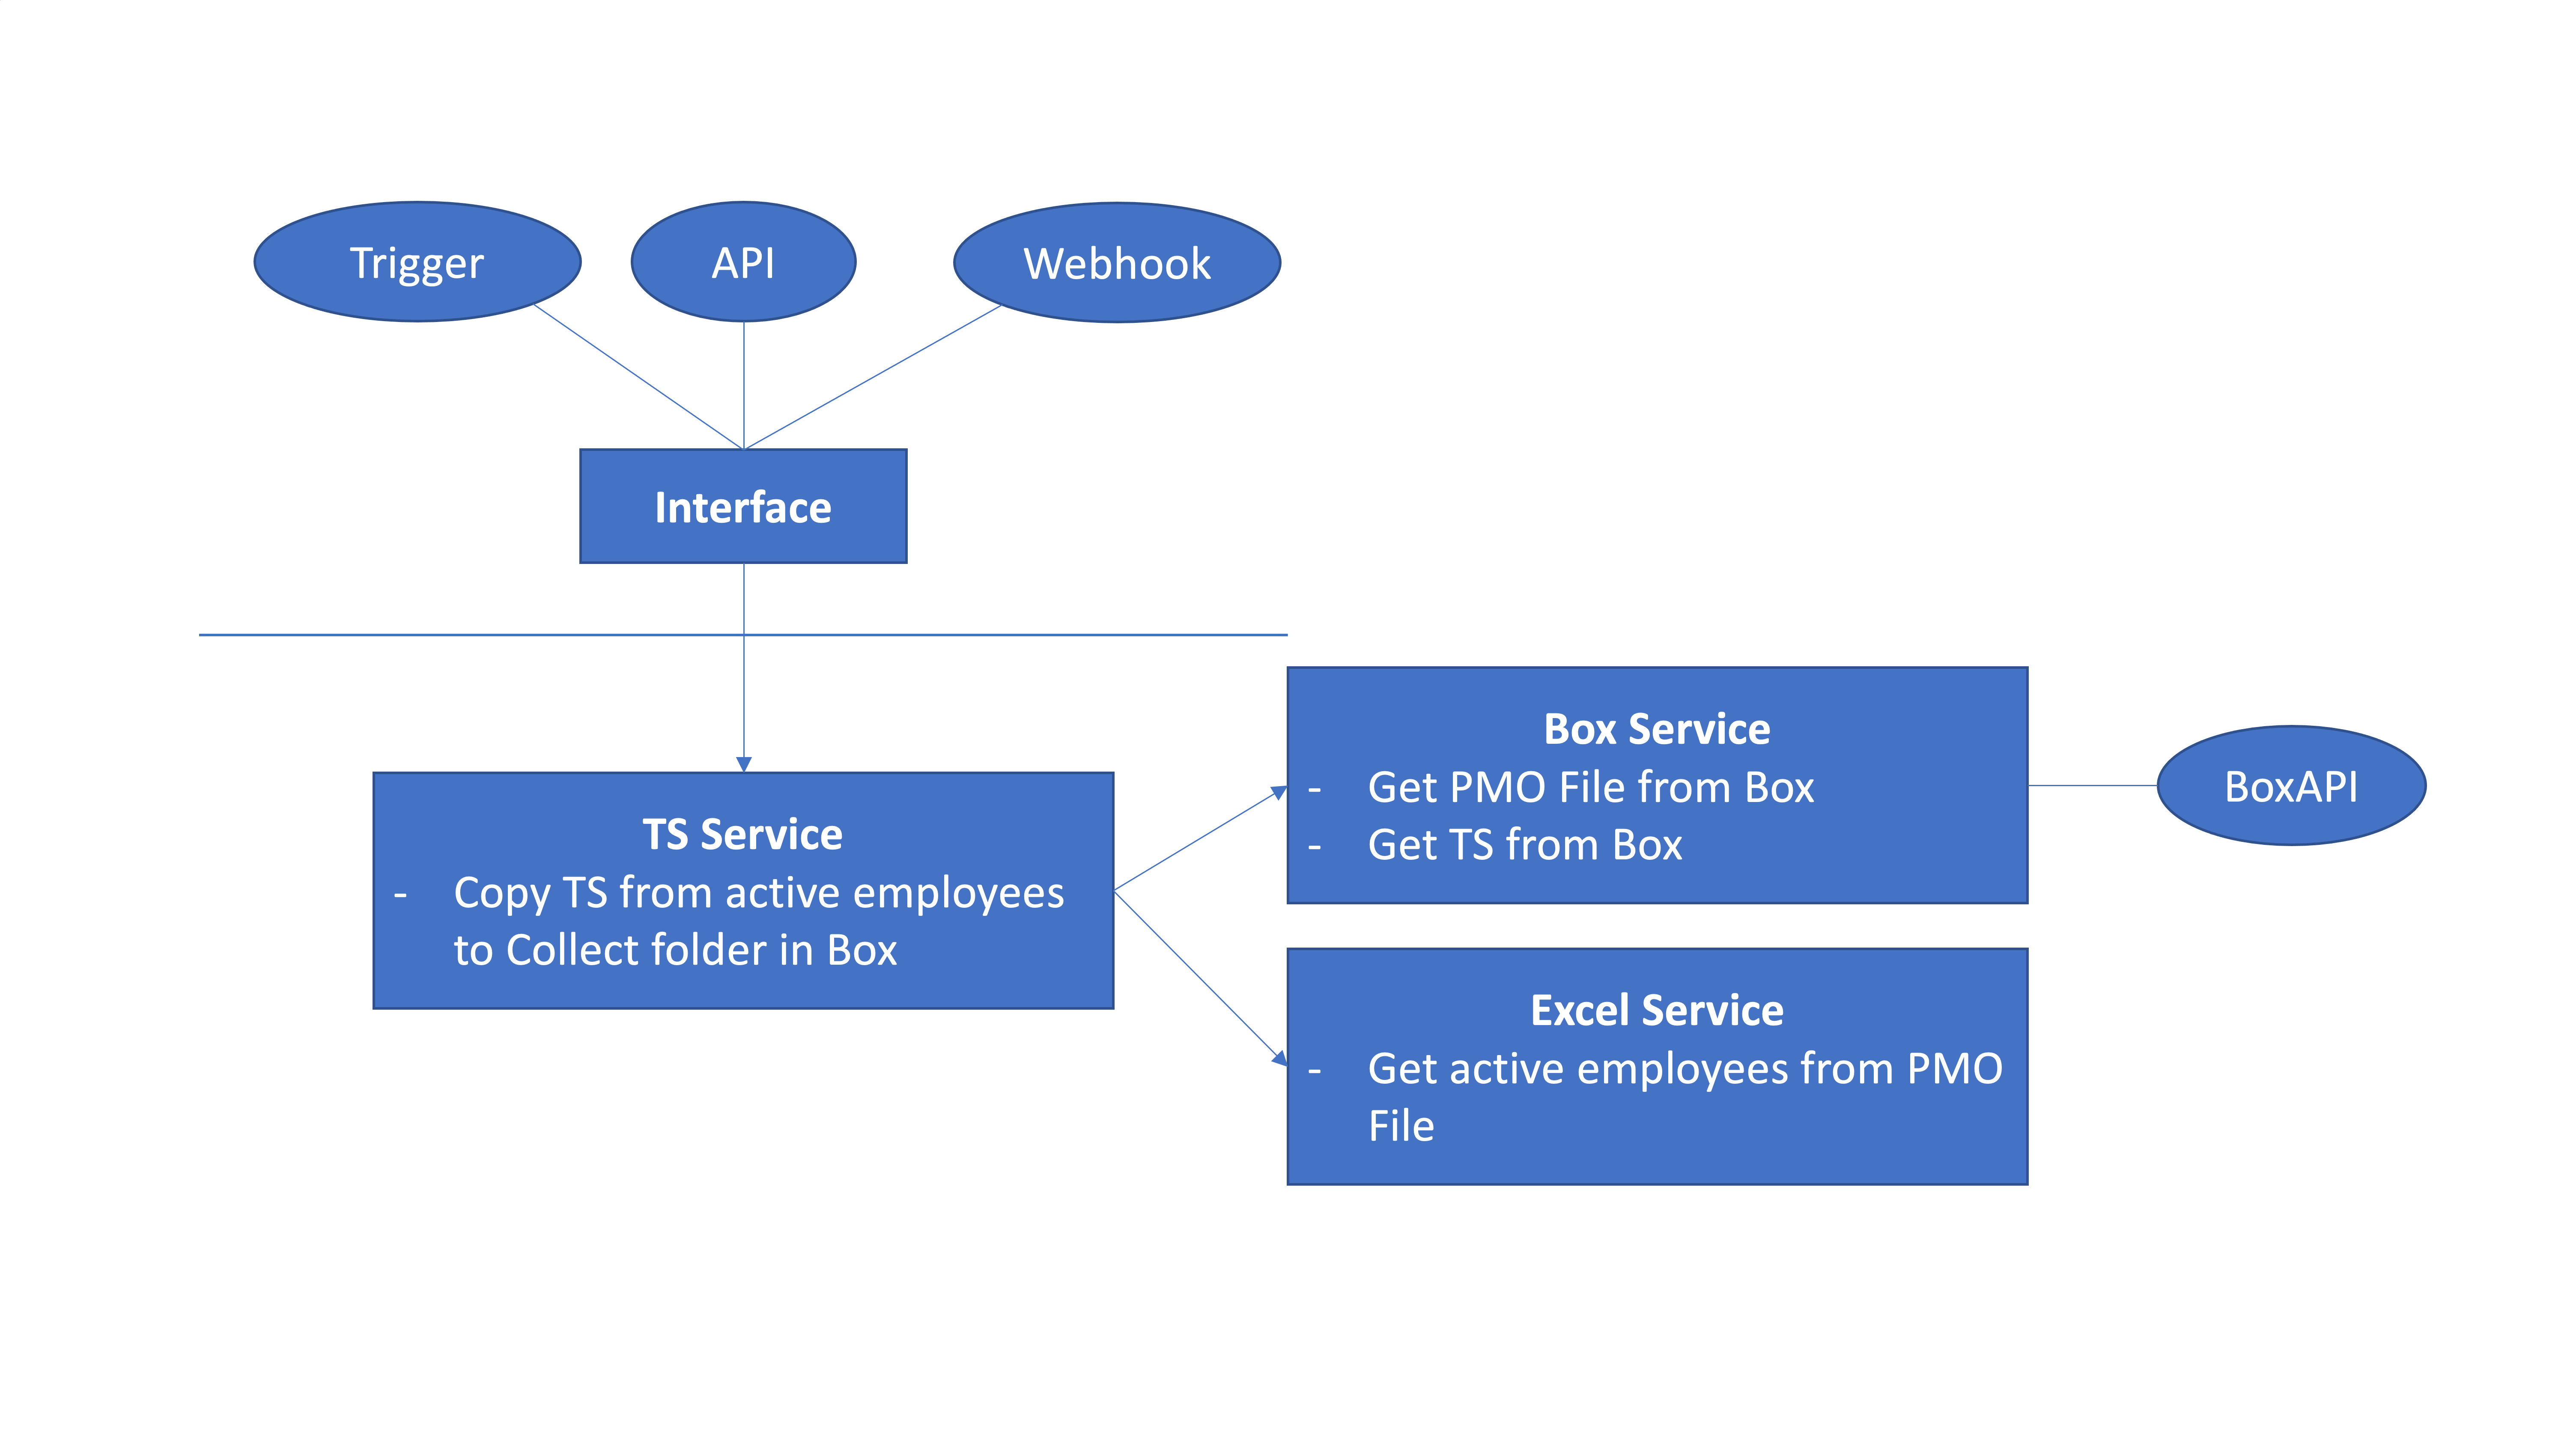
\includegraphics[width=\textwidth]{architektur.png}
    \caption{Grober Architekturentwurf}
    \label{fig:Architektur}
\end{figure}

Abbildung \ref{fig:Architektur} zeigt einen groben  Entwurf der Anwendung und wie die Services miteinander kommunizieren sollen. Der Timesheet Service soll zu einem späteren Zeitpunkt alle Funktionen aus der Ursprünglichen Anwendung bündeln, für den Prototypen wird sich jedoch, wie bereits in der Anforderungsanalyse erwähnt, auf den Collect Service beschränkt.

\subsection{Konzeptionierung der Services}
In der ursprünglichen Anwendung ist der Zugriff auf die \gls{Box} mithilfe der Box Drive Erweiterung umgesetzt worden. Diese ermöglicht es, Verzeichnisse in der \gls{Box} wie einen lokalen Dateipfad ansprechen zu können, zum Beispiel \textit{C:/Users/User/Box/Folder}. Somit konnte der Box-Pfad in eine Konfigurationsdatei geschrieben und als Parameter an die Anwendung übergeben werden. Nachteil an dieser Umsetzung ist die Notwendigkeit den \gls{Box}-Pfad anpassen zu müssen, wenn ein anderer Nutzer die Anwendung startet. Eine Einbindung der \gls{Box} \ac{API} für den Prototypen wird aus diesem Grund unumgänglich sein.

Der \gls{Box} Service muss Dateien herunterladen, die Inhalte von Ordnern auflisten und Ordner IDs ermitteln können.

Außerdem enthalten die PMO-Tools ein \glqq{excelhelper.py}\grqq{} Skript, welches den Umgang mit Excel Spreadsheets ermöglicht. Dazu gehört zum einen das Ermitteln aktiver Mitarbeiter und zum anderen das Auslesen der Timesheets, was jedoch für den Prototypen keine Verwendung findet. Einen vergleichbaren Service muss auch die neue Anwendung enthalten. Für Java kann man in diesem Fall auf die Apache POI Programmbibliothek zurückgreifen, welche das Lesen und Schreiben von Microsoft Office Dateien ermöglicht.

Den \glqq{Hauptservice}\grqq{} der Anwendung soll der Timesheet Service bilden. Dieser soll alle Funktionen bereitstellen, die unter Verwendung der anderen Services die letztendlich gewünschte Funktionalität des Einsammeln der Timesheets bieten. Darüber hinaus soll dieser für eine Spätere Anwendungsversion auch die anderen Funktionalitäten aus der ursprünglichen Anwendung bereitstellen. Dieser Service soll zu einem Späteren Zeitpunkt immer dann getriggert werden, wenn eine neue Konfigurationsdatei in einen entsprechenden \gls{Box} Ordner geladen wird. Für den Prototypen reicht jedoch ein simpler Trigger oder der Start via \ac{API} \textit{Request} aus. \textbf{TODO: Rephrasing und detaillierte Beschreibung der Architektur (welche Dienste werden benötigt)}\pagebreak

\subsection{Programmiersprache und Framework}
Neben der Konzeptionierung einer Anwendungsarchitektur braucht es zur Entwicklung auch eine Programmiersprache und gegebenenfalls ein Framework, um die Anwendung sinnvoll umzusetzen. Im Falle der PMO-Tools wurde ursprünglich Python verwendet, jedoch erschien im Zuge des Refactoring ein Wechsel zu Java und dem \gls{Spring} Framework sinnvoll. Aus diesem Grund wird auf \gls{Springboot} zurückgegriffen, zur vereinfachten Entwicklung von \gls{Spring} Anwendungen. \gls{Springboot} erleichtert die Cloud native Entwicklung. \textbf{TODO: Vorteile von Springboot}

\subsection{Auswahl eines Cloud Providers}
Ein für die Cloud Migration unerlässlicher Schritt ist die Auswahl eines zu den Anforderungen passenden Cloud Providers. In diesem Fall wurde \ac{AWS} als einer der größten Provider gewählt, da hier mit \ac{ECS} und Fargate gute Cloud native Möglichkeiten zum Deployment von Containern zur Verfügung stehen. Alternativ wurden auch die Services der IBM-Cloud in Betracht gezogen, da auch hier die entsprechenden Services existieren. \pagebreak